% * Embedded Systems domains are diversifying
%   => rise of non-experts using embedded systems
%   => IoT innovators / SMEs building new product
%   => Educators and Students

\section{Introduction}
\label{sec:intro}

Embedded systems are growing impressively in popularity and ubiquity in recent years. This growth can be attributed to the emergence of new application domains inspired by small, highly resource-limited programmable processors known as microcontroller units (or MCUs), which may have as little as a few kilobytes of RAM. With the growth in demand for a wide variety of systems, ranging from wearables, to home automation, industrial automation, and smart grids - a phenomenon broadly referred to as the Internet of Things (IoT) - it is now the case that less than 1 percent of the world's processors reside in general purpose computers such as desktop PCs, laptops and tablets - with MCUs picking up the remainder~\cite{borriello2000embedded}.

As the IoT has grown, it has become more pervasive, accessible, and generalised. Hence there has been a large growth in \emph{non-expert} developers using embedded systems to interact with other devices and objects. These devices have entered: the classrooms of educators as \emph{physical computing} devices; the workshops of hobbyists as \emph{maker} devices; and the hands of small to medium sized business as \emph{prototyping} devices. However, these new developers share a common characteristic - \emph{they are typically not professional software developers}~\cite{dougherty2012maker,bruce2015make,maksimovic2014raspberry}.

Figure~\ref{fig:projects} shows an example of some of the projects \emph{non-experts} create. A key observation here is that these projects require \emph{non-trivial engineering skills}: to record the temperature in space over time, one must log data to flash for extraction at a later date; to report telemetry of a rocket car, one must use Bluetooth to communicate from the embedded system, to a stationary device for visualisation.

It is important, as embedded software engineers, that we engage with, and encourage this demographic to explore embedded systems.

\begin{figure}[t]
    \centering
    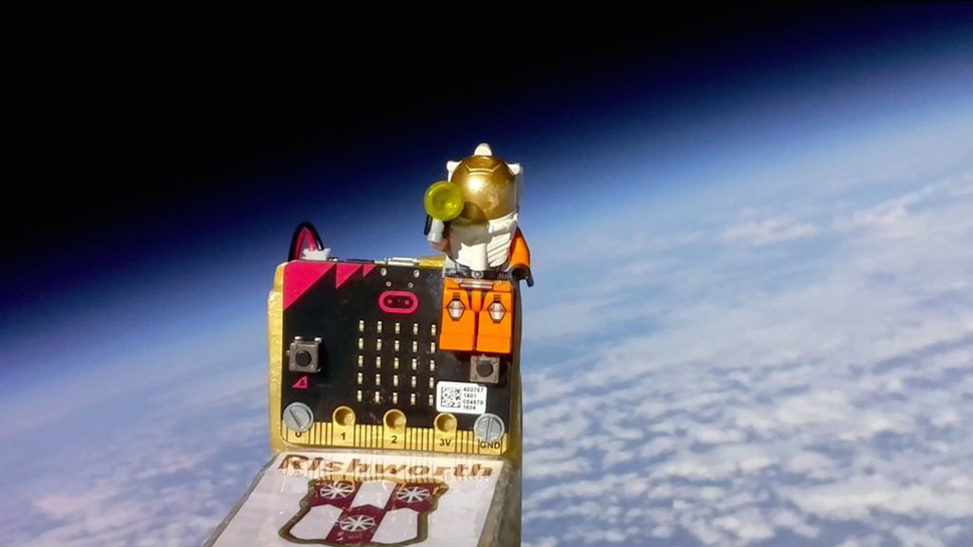
\includegraphics[width=.49\columnwidth]{images/microbit-space.jpg}
    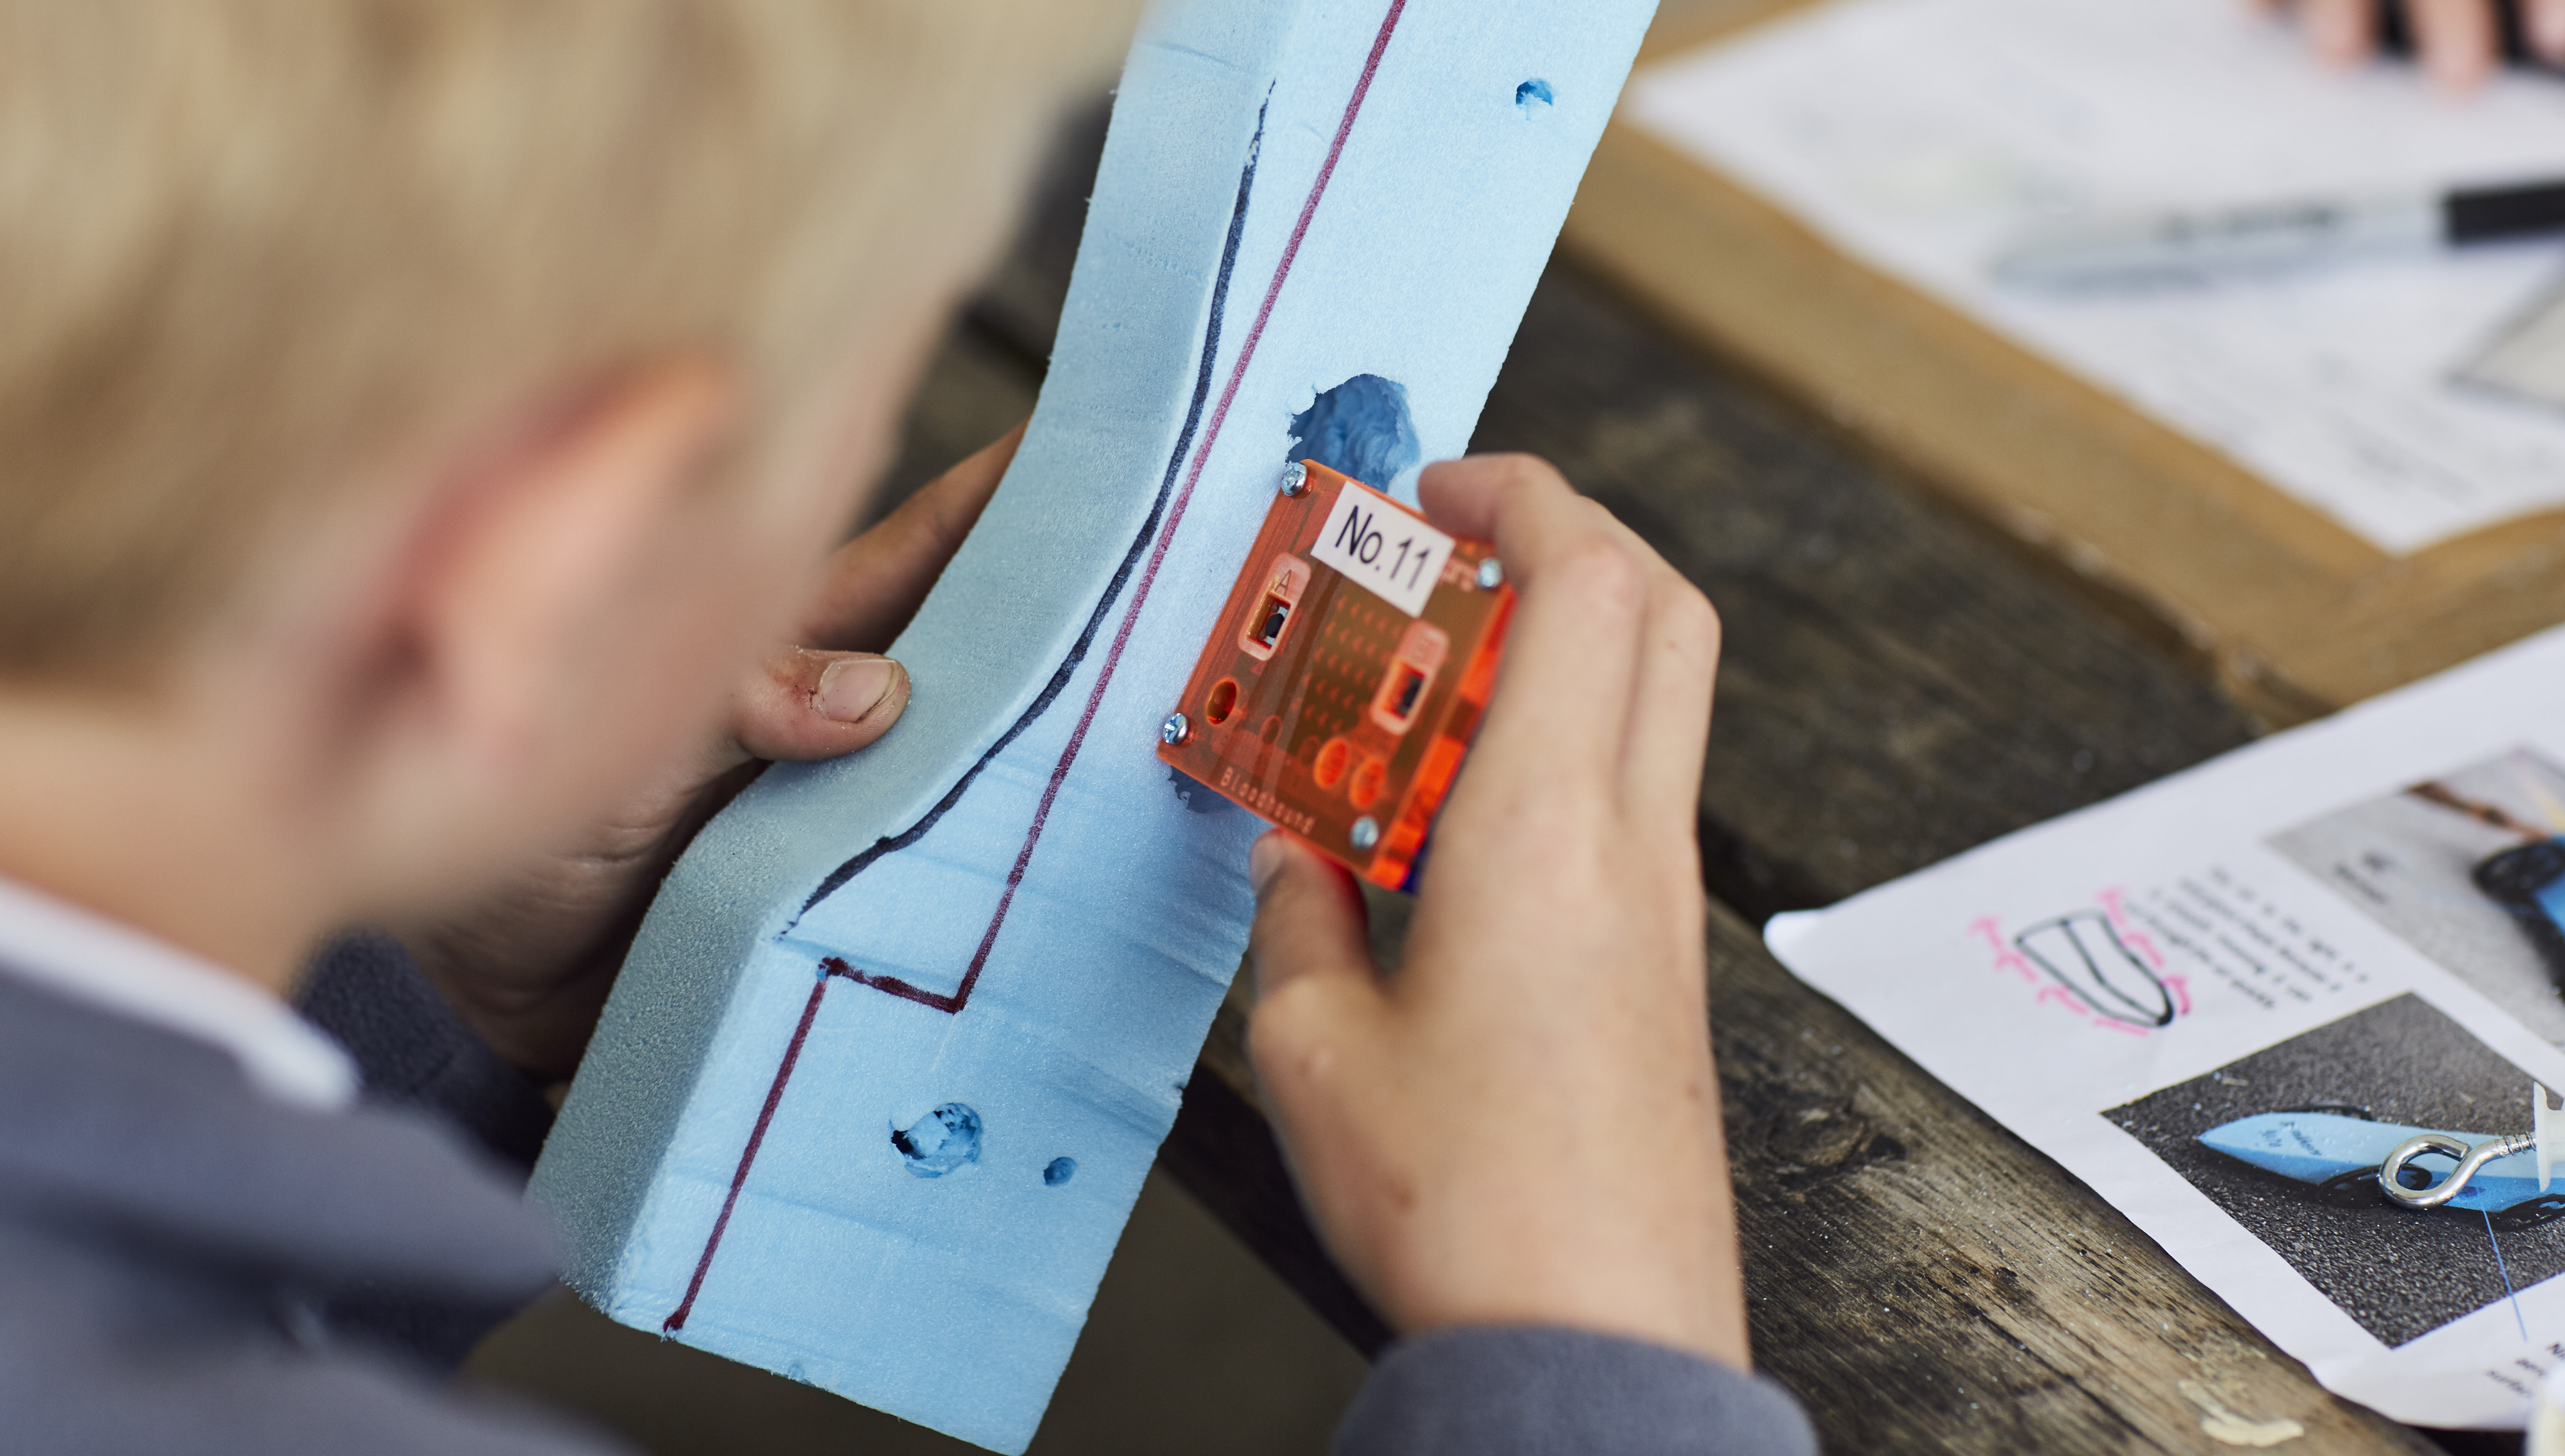
\includegraphics[width=.49\columnwidth]{images/bloodhound.jpg}
    \caption{\label{fig:projects} Projects created by non-experts: Rishworth School sent a micro:bit to space (left); and other placed the micro:bit in a custom-built rocket car for telemetry (right); }
\end{figure}

\subsection{Background}
\label{sec:background}

In continuum, we make key observations on the current design of the embedded Internet of Things for non-expert developers, including: the hardware, the programming languages and the environments in use.



\begin{table}[]
    \centering
    \begin{tabular}{|l|r|r|r|r|r|r|}
    \hline
                           &          &              & \bf{Word}  & \bf{CPU} &            \\
    \bf{Device}            & \bf{RAM} & \bf{Flash}   & \bf{Size}  & \bf{Speed} & \bf{CPU}  \\ \hline
    Uno            & 2 kB       & 32 kB      & 8          & 16MHz & AVR       \\ \hline
    micro:bit          & 16 kB      & 256 kB     & 32         & 16MHz & Cortex     \\ \hline
    CPX           & 32 kB      & 256 kB     & 32         & 48MHz & Cortex    \\ \hline
    PC             & 16 GB      & 1 TB       & 64         & 3GHz & Intel      \\ \hline
    \end{tabular}
    \caption{\label{table:devices}Example microcontroller devices in relationship to a typical PC. Device abbreviations: Uno (Arduino Uno), micro:bit (BBC micro:bit), CPX (Adafruit Circuit Playground Express); PC (Personal Computer).}
\end{table}

\paragraph{MCUs are processor rich, but memory scarce}
Table~\ref{table:devices} compares the core capabilities of the class of MCU-based devices used by non-experts to a typical PC. Contrary to first impressions, these devices have a \emph{proportionally} large amount of processing power. Consider the BBC micro:bit versus a typical PC. It has about 100 times less CPU power, but 10\textsuperscript{6} times less RAM, and 10\textsuperscript{6} times less storage.

\paragraph{MCUs are feature rich} MCUs still follow Moore's law (the number of transistors doubles roughly every two years). However, this additional capacity is not typically invested in simply optimizing processing power. Instead, \emph{independent peripherals} are integrated onto the same MCU as the CPU. Examples include integrated radio hardware such as Bluetooth/WiFi and audio inputs and outputs.

\paragraph{Programming languages are too complex}
Programming languages for MCUs have not kept pace with advances in hardware and diversification of user domains. In the world of the MCU, the C/C++ languages remain the standard, and for good reasons: they provide a familiar imperative programming model, with compilers that produce highly efficient code, and enable low level access to hardware features when necessary. Popular examples include the Arduino project (\url{www.arduino.cc})~\cite{buildingArduino2014}, started in 2003, and ARM's Mbed platform (\url{www.mbed.org})~\cite{ARMmbed} --- both of which rely heavily on a C/C++ programming model. However, the limitations of using C/C++ as an application programming language for \emph{inexperienced} developers are well understood~\cite{blikstein2013gears}. To address this, others have ported lightweight versions of virtual machines for popular higher level languages like Python, Java, and JavaScript, to this class of MCU. However, these languages prove difficult for novice programmers and consume a large amount resources, sometimes detrimentally.

\paragraph{Programming environments are too integrated}
To create and transfer programs to accompanying hardware, programs, drivers, and toolchains must be installed. For \emph{non-experts}, installation of software can be a difficult task, and impossible in some environments due to restrictions placed on machines.


\subsection{Requirements}
\label{sec:requirements}

From our observations we derrive the following requirements for a platform suited to this new demographic:

\begin{enumerate}

    \item To facilitate engaging educational scenarios and to enable exciting IoT projects, an abstraction layer should effectively hide unnecessary complexity, and actively expose interesting features of the hardware.

    \item With memory scarce MCUs, a language/runtime should therefore not only seek to provide high code density and spatial efficiency, \emph{but to actively trade off time for space}, where possible.

    \item Due to feature rich hardware, an effective language/runtime should directly support \emph{an asynchronous interaction model} designed to cooperate with the independent nature of peripherals.

    \item To engage with all demographics, there is a need for \emph{an asynchronous programming language for embedded systems}, that lowers the barrier to entry, whilst maintaining temporal and spacial efficiency.

    \item With the diverse, non-expert demographic, the ability to \emph{create and transfer programs without installing any additional software} is vital.

\end{enumerate}

This paper focuses on the design, implementation, and evaluation of a new web-based development environment, language, and runtime, using the devices listed in Table~\ref{table:devices}. More specifically, we present and evaluate a platform that bridges the worlds of the web and the MCU through two novel technologies:

\begin{itemize}
\item \emph{\MCN}, a no-install web-based application containing an \emph{in-browser compiler} that supports the simplified asynchronous programming of MCUs via editors for visual blocks and textual JavaScript languages (Section~\ref{sec:makecode});

\item \emph{\CO} which contains: (1) a component-oriented, event-driven, fiber-based C++ runtime environment that bridges the semantic gap between higher-level languages (such as TypeScript) and the hardware, modelling each hardware component as a software component (Section~\ref{sec:codal});  and (2) \emph{\UF}, a new file format for simplified transfer of serial data (such as programs) to the device, using a driverless USB mass storage abstraction (Section~\ref{sec:uf2});

\end{itemize}

Our results (Section~\ref{sec:evaluate}) show that these technologies combined can enable simplified programming through modern languages and event-based constructs while maintaining a relatively high degree of temporal and spatial efficiency. We demonstrate up to 50x better performance than other state-of-the-art implementations,
in some cases nearing the performance of native C++.

% Our platform was deployed about a year ago at \url{www.makecode.com} and sees daily use by thousands of users.

% * Derive Requirements

% => Modern IoT Hardware
%     => Low cost
%     => 32 bit processor rich, ram poor MCUs
%     => Async h/ware

% => Universality

%   => Modern High level Langaguges
%     => Blocks
%     => Typescript
%     => C++
%     => Low barrier to entry
%     => Without sacrificing capability
%       => Temporal Efficiency
%       => Spacial Efficiency
%     => Async (HL languages are Async and the hardware is moving that way)
%     => First class Event support

%   => Modern Toolchains
%     => Universal Web based UI
%     => Driver free wired/wireless device integration

% * Paper Overview
% - background
%    - examples of awesomeness in the classroom, breaks the mould, not just blinking an LED
%    - scale
%    - non-trivial, engineering.
% - architecture
%    - makecode
%       - under the compiler section, mention no VM
%    - codal
%      - codal is not an RTOS
%    - uf2
% - eval
% - R/W
% - conclusions


% The emergence of a new breed of computer




% MCUs are highly resource limited devices, but are not simply smaller versions of laptop and desktop machines. They are architecturally quite distinct. If we are to understand how to optimize programming languages and their implementation for such devices it is worth dwelling on the key characteristics of MCUs, namely their storage and CPU capabilities. Table \ref{table:devices} highlights the core capabilities of MCU-based devices vs. a typical PC.


% While such devices are highly resource constrained compared to modern PCs (about six orders of magnitude less on some metrics), a deeper analysis derives two further observations.

% Firstly, \emph{MCUs are processor rich}. Contrary to first impressions, these devices have a \emph{proportionally} large amount of processing power. Consider the BBC micro:bit versus a typical PC. It has about 100 times less CPU power, but 10\textsuperscript{6} times less RAM, and 10\textsuperscript{6} time less storage. A language/runtime designed for MCUs should therefore not only seek to provide high code density and spatial efficiency, \emph{but to actively trade off time for space}, where possible.

% Secondly, \emph{MCUs are accumulating more features on chip}. MCUs still follow Moore's law (the number of transistors doubles roughly every two years). However, this additional capacity is not typically invested in simply optimizing processing power. Instead, \emph{independent peripherals} are integrated onto the same MCU as the CPU. Examples include integrated radio hardware such as Bluetooth/WiFi and audio inputs and outputs. This hardware is designed to run independently of the CPU, hence an effective language/runtime should directly support \emph{an asynchronous interaction model}.

% % move to education
% % educators hate barriers
% % existing barriers
% % there are new devices with more functionality released to schools, yet these still suffer from historic problems with compilation toolchains and installation and programming, their CPUs are highly capable but under resourced. How do you do high level languages, no installation, lots of educational value with no resources.
% % we aim to solve x with our platform.
% Furthermore, with the increased embedding of technologies into our everyday lives, it is important that future generations are educated, can use, and fully understand the technologies around them. To enhance the learning of their students, educators have begun to introduce embedded systems into the classroom, creating a cohort of new application developers. These new developers share a common characteristic - \emph{they are typically not professional software developers}~\cite{dougherty2012maker,bruce2015make,maksimovic2014raspberry}.

% From our prior experience in this domain, we recognise three concerns that educators have when considering a physical computing device:
% \begin{enumerate}
%     \item \emph{Ease of integration} - The embedded system must be easy to integrate into the classroom, any overhead of configuration or installation will likely meet resistance from the IT support staff within a school;
%     \item \emph{Learning curve} - Educators and their students are not computer scientists, and have very little time outside of their working day to explore new technologies, therefore the embedded system needs to be easy to understand, program, and use;
%     \item \emph{Cost \& educational value} - The cost of the embedded system must be low, yet provide enough educational value to justify the purchase to a school;
% \end{enumerate}

% Programming languages and development environments for MCUs have not kept pace with advances in hardware and diversification of user domains. In the world of the MCU, the C/C++ languages remain the standard, and for good reasons: they provide a familiar imperative programming model, with compilers that produce highly efficient code, and enable low level access to hardware features when necessary. Popular examples include the Arduino project (\url{www.arduino.cc})~\cite{buildingArduino2014}, started in 2003, and ARM's Mbed platform (\url{www.mbed.org})~\cite{ARMmbed} - both of which rely heavily on a C/C++ programming model. However, the limitations of using C/C++ as an application programming language for \emph{inexperienced} developers are well understood~\cite{blikstein2013gears}. Further, the hardware accompanying these platforms require additional software installation to operate.

% Paper overview
% We introduce a novel architecture for MCU-based devices, that:
% requires no installation, to ease integration
% offers high level programming languages, to reduce the learning curve
% provide

% This paper focuses on the design, implementation, and evaluation of this architecture using the devices listed in Table~\ref{table:devices} as exemplars. We leave a detailed treatment about usability for future work. More specifically, we present and evaluate a platform that bridges the worlds of the web and the MCU through three novel technologies:

% \begin{itemize}
% \item \emph{\MCN}, a web application containing an \emph{in-browser compiler} that supports the simplified programming of MCUs via editors for visual blocks and textual JavaScript languages (Section~\ref{sec:makecode});

% \item \emph{Static TypeScript}, a statically-typed subset of TypeScript (\url{www.typescriptlang.org}) that we have defined for fast execution on low-memory devices, with a simple model for linking against pre-compiled C++ (Section~\ref{sec:sts});

% \item \emph{\CO}, a component-based, event-driven, fiber-based C++ runtime environment that bridges the semantic gap between higher-level languages (such as TypeScript) and the hardware, modelling each hardware component as a software component (Section~\ref{sec:codal});
% \end{itemize}

% Our results (Section~\ref{sec:evaluate}) show that these technologies combined can enable simplified programming through modern languages and event-based constructs while maintaining a relatively high degree of temporal and spatial efficiency. We demonstrate up to 50x better performance than other state-of-the-art implementations,
% in some cases nearing the performance of native C++. Our platform was deployed about a year ago at \url{www.makecode.com} and sees daily use by thousands of users.

%\subsection{Open Source Repositories}
%\input{open}